% !TEX root = ../main.tex

\chapter{相干首波}

\section{声速的测量}

任何合格的物理本科生都熟悉如何在空气或水中测量声速,如共振波节法、相位法、时差法。前两者的原理都是寻找固定频率信号的某个特殊相位(如峰值所对应的 $\uppi/2 + 2n\uppi$,$n\in\mathbb{Z}$)下的空间位置,从而通过逐差法确定声波的波长;后者则是考虑到了声学探头中压电陶瓷进行声-电转换所需要的固有时间,因此通过拟合空间位置与到达时间的斜率以确定声速。事实上,在颗粒固体中测量声速时,上述方法都有不同程度的应用,如 Paul A.Johnson 和 Xiaoping Jia 同时使用共振法与行波法(即飞行时间法,Time of Flight, T.O.F.)测定颗粒介质中的声速\cite{Johnson_2005};而在地震学中,基于连续小波变换(Continuous Wavelet Transform, CWT)和频散能量图求解地震波相速度的方法也被广泛应用。本节将介绍如何使用飞行时间法与频散能量图测量颗粒介质中的声速。

\subsection{装置搭建}

目前部署的声学探测与激励系统部件如下:

\begin{itemize}
  \item Tektronix Arbitrary Function Generator AFG31021。该仪器可以按照实验需求产生如连续正弦波、某循环数正弦波列、单频脉冲等电压信号,用于激励声学探头产生对应机械振动。其支持写入自定义函数来对信号波形进行控制;
  \item Tektronix TBS2204B 示波器。该示波器通过 BNC 接口对多达 $4$ 个独立模拟电压信号进行同步采集,可用于记录试探信号与在颗粒介质中传播后的响应信号。示波器的采样率最高可达 $1\unit{\giga\hertz}$,单次采样长度最高可达 $5\times 10^{6}$。通过 IPv4 网口可使用 TekScope 软件对 TBS2204B 进行数据读取和记录,并且进行简单程度的操控(开始/停止记录)等;
  \item ATA-101B Power Amplifier。可以设置输入与输出的线缆阻抗(目前声学常用线缆都是 $50\unit{\ohm}$),其主要功能是以最小步长 $2\unit{\decibel}$ 放大 AFG31021 产生的电压信号,从而使声学探头产生更高需求的声压振幅,通常适用于有限振幅波传播的非线性等实验中。可设定的最大放大效果为 $20\unit{\decibel}$,但是由于其固有的频域放大极限,如果初始输入的电压信号幅值已经较大,未必能完全做到这一点;
  \item 清诚声发射 G150 与 W800 (成对)声学探头。声学探头在相关领域中又被称为换能器(Transducer),即压电陶瓷既能够将射频线缆传输的模拟电压信号通过电-压效应转换为机械振动(声信号),又能够通过监测机械振动、通过压-电效应转换为模拟电压信号,从而进行进一步的信号处理与分析。G150 和 W800 分别是适用于 $60-400\unit{\kilo\Hz}$ 和 $50-800\unit{\kilo\hertz}$ 频域范围内工作的探头型号,应当根据实验需求选取合适的一对探头。两个型号的声学探头主体都是 $\varphi 19\unit{\milli\meter}\times 15\unit{\milli\meter}$ 的圆柱体,因此便于安装于同一颗粒容器中;
  \item 单轴应力圆柱容器。通过 SOLIDWORKS 软件设计并采用亚克力板制作的容器(采用透明容器是为了兼容未来可能的 X 射线扫描建模需求)。容器内径为 $D = 90\unit{\milli\meter}$, 最高支持厚度为 $13\unit{\centi\meter}$ 的颗粒介质进行实验。设置四轴活塞对容器内的颗粒介质施加单轴应力,活塞与容器底部中心均留有 $\varphi 19\unit{\milli\meter}$ 的孔洞用于安装声学探头。容器壁通过 $10\unit{\milli\meter}$ 的亚克力板弯曲为圆筒制作,因此可以承担实验需求范围的应力。探头和容器均未考虑防水/密封处理。
\end{itemize}

%%% 这里放实验装置部件的示意图

%%% 找到一个用 tikz 画工作流示意图的方法

需要说明的是,一般情况下作用于接收器表面的声压 $p(t)$ 都并不等于入射波的声压 $p_{i}(t)$,这是由探头的声阻抗 $\widetilde{Z}_{S}(\omega)$ 导致的:

\begin{equation}
  p(t) = \left(1 + \frac{\widetilde{Z}_{S}(\omega)}{\rho_{0}c_{0}S}\right) =\widetilde{K}(\omega)p_{i}(t).
\end{equation}

其中 $\rho_{0}$ 与 $c_{0}$ 是介质中平衡态下的密度和声速,$S$ 是圆面探测器的面积。接收声压 $p(t)$ 通过非幺正角频率傅里叶变换得到的频谱为

\begin{equation}
  F(\omega) = \int_{-\infty}^{+\infty}\widetilde{K}(\omega)p_{i}(t){\ee}^{-\ii\omega t}\mathrm{d}t = \widetilde{K}(\omega)F_{i}(\omega).
\end{equation}

其中 $F_{i}(\omega)$ 为入射波声压的非幺正角频率傅里叶变换。因此入射波声压 $p_{i}(t)$ 为

\begin{equation}
  p_{i}(t) = \frac{1}{2\uppi}\int_{-\infty}^{+\infty}\frac{F(\omega)}{\widetilde{K}(\omega)}{\ee}^{\ii\omega t}\mathrm{d}\omega\label{eq:response_correct}
\end{equation}

在实验中,由于我们使用的是一对同工作频域的探头,面对面接触时可以简单视为声波经历了两次同样的声阻抗过程,且假定压电效应呈现线性($p\propto U$)。那么,我们可以设定信号发生器产生的电压信号为 $U_{0}(\omega)$,则接收到的电压信号为

\begin{equation}
  U(\omega) = \widetilde{K}(\omega)^{2}U_{0}(\omega).
\end{equation}

图~\ref{fig:response_factor} 展示了设定源信号为一系列相同振幅、不同频率 $\omega_{n}$ 的连续正弦波列 $\{U(\omega_{n})\}$ 时测定的探头响应系数 $\widetilde{K}(\omega)$。

\begin{figure}[!htp]
  \centering
  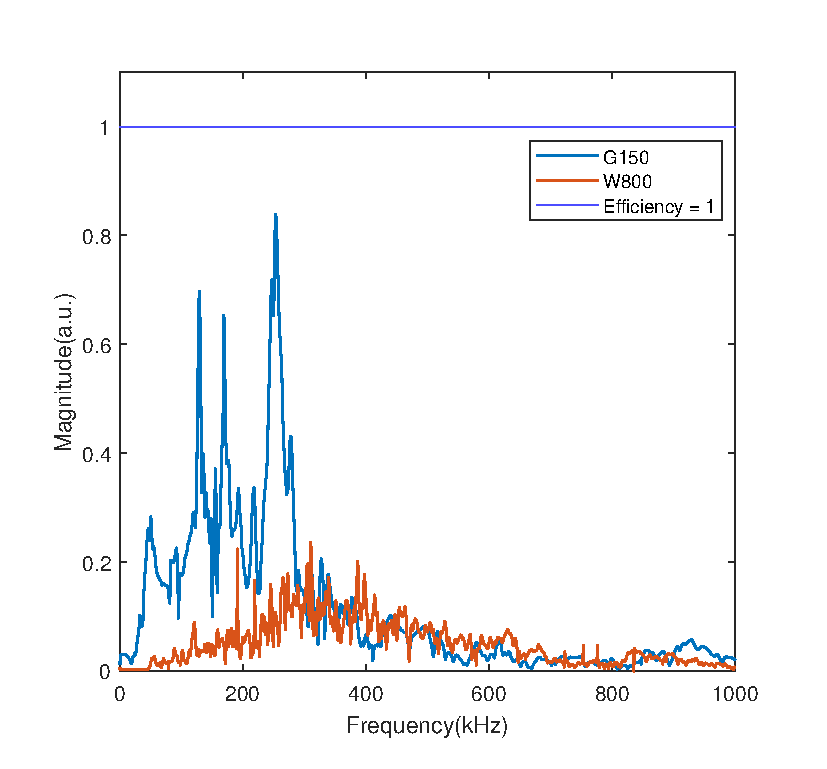
\includegraphics[height=8cm]{2_response_factor.eps}
  \bicaption{G150 与 W800 两种声学探头响应系数 $\widetilde{K}(\omega)$}{Response factor $\widetilde{K}(\omega)$ of G150 and W800 acoustic sensors}
  \label{fig:response_factor}
\end{figure}

观察可知,G150 在 \numrange{60}{400}\unit{\kilo\hertz} 频域内的响应系数非常接近 $1$, 而超出其工作频域的响应系数迅速跌落;而 W800 在我们关心的频域 \numrange{0}{1000}\unit{\kilo\hertz} 内虽然响应系数均不高,但是胜在响应曲线相对平稳。因此在实验时,如果信号集中于超声频域内的较低成分,那么选择 G150 将是更合理的;在关心较广的频域下的声学参数(比如衰减、相速度等)时,W800 的性能相对优异。为了弥补 W800 本身响应系数较低的缺陷,未来可以考虑使用 Physics of Acoustic Company 的 2/4/6 Type 等前置放大器来对有效信号进行增强。

我们后续实验便可以借助式~\eqref{eq:response_correct} 来对实验中采集的响应信号进行修正,这对幅值相关的声学测量实验意义重大。

\subsection{飞行时间法测定颗粒介质中的声速}

飞行时间法测定声速的原理即测量试探声波从声源探头到接收探头的时间差 $\Delta t$,从而计算得到

\begin{equation}
  V_{\text{T.O.F.}} = \frac{L}{\Delta t}.
\end{equation}

其中 $L$ 是颗粒介质的厚度。但是如何准确定义声波的到达时间(Arrival Time)是值得商榷的问题。Ellák Somfai 等人定义颗粒介质中声波的三种不同的到达时间:波前到达时间 $t_{0}$(由于噪声的存在,波前通常被定义为上升沿峰值 $A_{1}$ 的 $\num{10}\%$ 处,部分更激进的研究者会选取为 $3\%$),波峰到达时间 $t_{1}$,首次过零时间 $t_{2}$\cite{PhysRevE.72.021301}。良好定义的波速应当满足在不同厚度下测得的结果相近,因此我们可以按照其确定在使用飞行时间法测定声速时的最佳信号参考点。

%%% 这里放参考文献的三个不同到达时间的示意图

\subsubsection{信号最佳参考点选取}

我们在实验中使用 Tektronix 示波器对源信号与响应信号进行了同步采集,因此容易确定具体的时间起点。基于调整噪声阈值、最小半高宽等参数的寻峰算法,我们可以准确定位源信号的峰值,从而根据因果关系筛去可能错误识别的噪声。图~\ref{fig:reference_point}是对典型的响应信号进行三种不同到达时间识别的实例。


\begin{figure}[!htp]
  \centering
  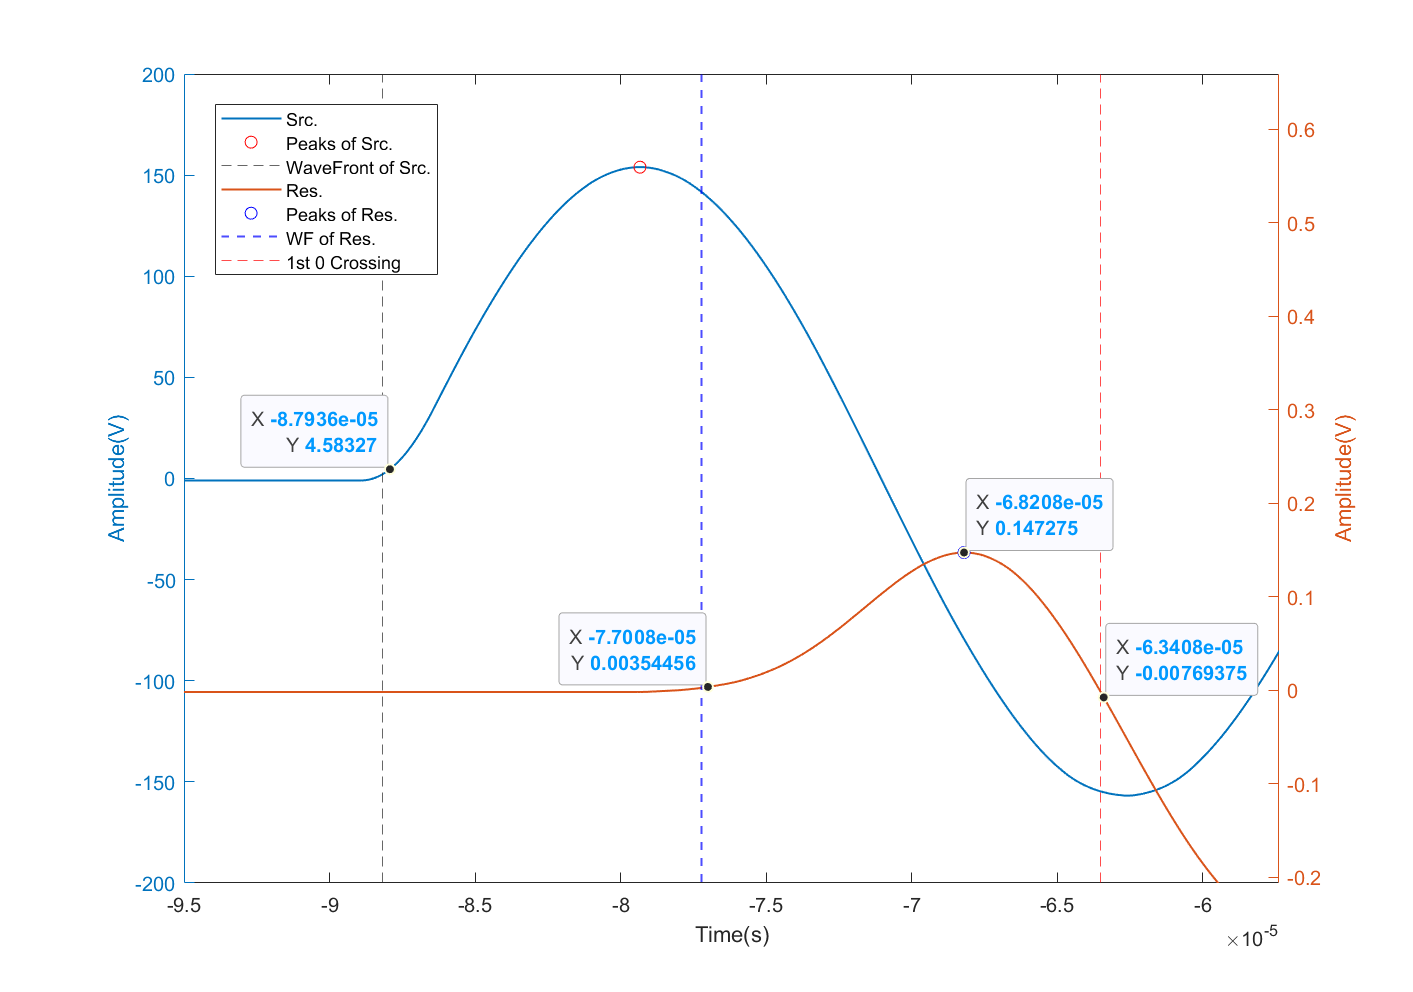
\includegraphics[height=8cm]{2_reference_point.png}
  \bicaption{同步采集源信号与响应信号,以及波前到达时刻,波峰到达时刻与首次过零时刻}{Synchronized acquisition of source and response signals, as well as wavefront arrival, peak arrival and first zero crossing moments}
  \label{fig:reference_point}
\end{figure}

我们按照上述三种到达时间的识别方法,测定了在不同厚度下的声速。特别地,我们额外使用时差法拟合得到了声速 $V_{L}$,并将其与飞行时间法测定的声速 $V_{\text{T.O.F.}}$ 进行比较。结果如图~\ref{fig:sound_velocity_measurement} 所示。实验中所使用的颗粒为 $d=2\unit{\milli\meter}$ 的钢珠,施加的单轴应力为 $P=9\unit{\kilo\Pa}$,试探信号设定为 $5$ 循环 $30\unit{\kilo\Hz}$ 正弦波列。每一个厚度都重新制备 $7$ 个不同的随机密堆积以进行系综平均,从而尽可能消除颗粒介质本身随机性的误差。

\begin{figure}[!hbtp]
  \centering
  \bisubcaptionbox{以三种参考点通过时差法求得的声速 $V_{L}$}%
                  {Sound velocity $V_{L}$ measured by time difference method with three reference points}%
                  [6cm]{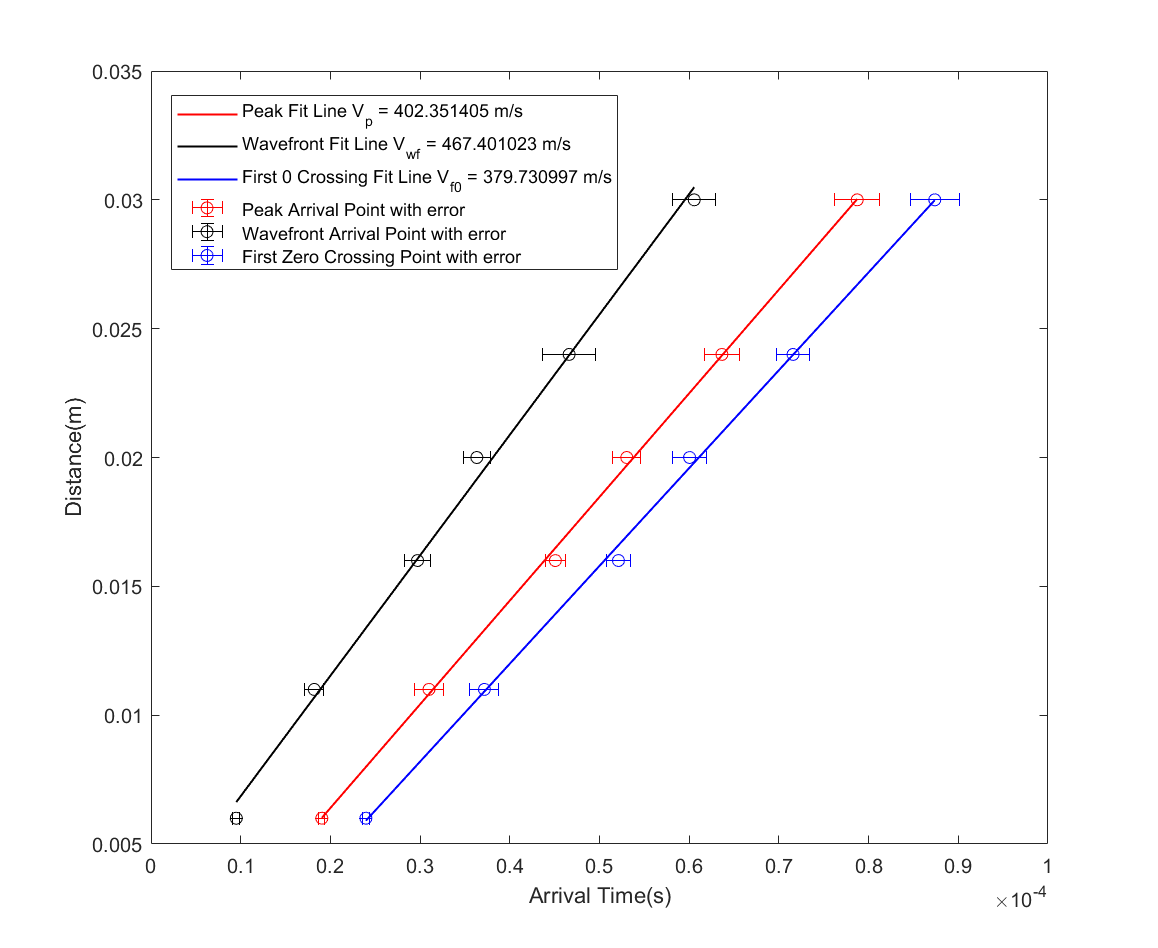
\includegraphics[height=6cm]{2_fitted_velocity.png}}
  \hspace{1cm}
  \bisubcaptionbox{以三种参考点通过飞行时间法求得的声速 $V_{\text{T.O.F.}}$}%
                  {Sound velocity $V_{\text{T.O.F.}}$ measured by Time of Flight method with three reference points}%
                  [6cm]{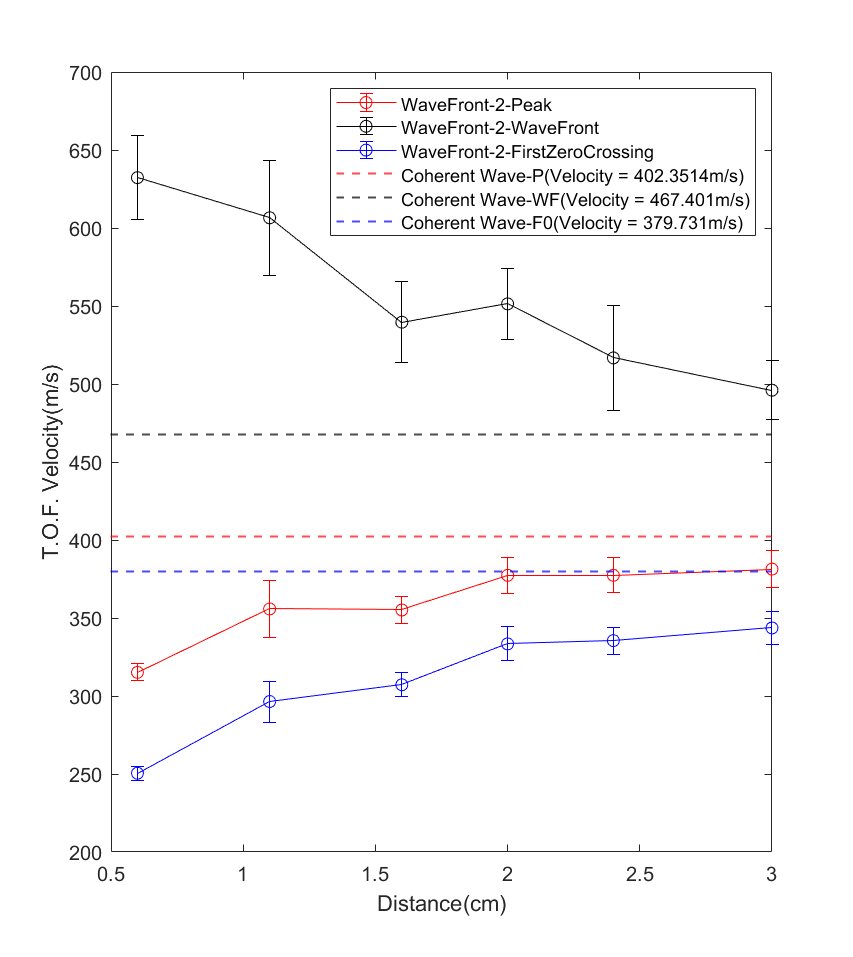
\includegraphics[height=6cm]{2_tof_velocity_and_fitted_velocity.png}}
  \bicaption{$5$ 循环 $30$ 千赫兹正弦波列作为试探信号,颗粒介质为直径 $2$ 毫米钢珠的随机密堆积,单轴应力 $9$ 千帕下的声速测量}
            {Velocity of sound measurements at $9\unit{\kilo\Pa}$ uniaxial stress with $5$-cycle of a $30\unit{\kilo\Hz}$ sine wave train as a test signal and a randomized stack of $2\unit{\milli\meter}$ diameter steel beads as the granular medium}
  \label{fig:sound_velocity_measurement}
\end{figure}

由此可见,各参考点的飞行时间法定义下的声速随着传播距离 $L$ 的增大向其时差法定义下的声速 $V_{L}$ 逼近,其中以波峰到达时间 $t_{1}$ 定义的声速在距离上的变化最为稳定,因此在传播距离足够大时,我们可以使用飞行时间法替代时差法进行工程上的声速测量,而其中以波峰到达时间定义的又是最好的。

需要额外说明的是,不同的参考点对于时差法都可以适用,但是其大小顺序和参考点的时间顺序明显相关,我们将其概括为相干首波在颗粒介质中随着传播距离增大而出现的展宽,即颗粒介质中出现了色散现象;我们将在后文通过归一化宽度更详细地探讨这一点。

% \begin{figure}[!hbtp]
%   \centering
%   \subcaptionbox{健康/损伤信号}%
%                 [7cm]{\includegraphics[height=6cm]{figures/signal_1.png}}
%   \hspace{1cm}
%   \subcaptionbox{散射信号}%
%                 [7cm]{\includegraphics[height=6cm]{figures/signal_2.png}}
%   \caption{响应信号处理}
%   \label{fig:bisubcaptionbox}
% \end{figure}

\subsection{频散能量图法}

\subsubsection{测量相速度的原理推导}

如果我们将颗粒介质中的声学传播简单考虑为单频平面波,即

\begin{equation}
  s(x,t) = A_{0}{\ee}^{-\alpha x}{\ee}^{\ii(\omega x/V_{\varphi}-\omega t)},
  \label{eq:spherical_wave}
\end{equation}

考虑在距离声源 $x_{1}$ 与 $x_{2}$ 处的两个接收探头,分别接收到声波信号 $S_{1}(t)$ 与 $S_{2}(t)$。则能求解相速度为

\begin{equation}
  V_{\varphi} = \frac{x_{2}-x_{1}}{\Delta \varphi}\omega.
\end{equation}

我们很容易想到通过 FFT 算法求解两次信号的相位频谱 $\varphi_{i}(\omega)$, 但是显然

\begin{equation}
  \Delta \varphi = \varphi_{2}(\omega) - \varphi_{1}(\omega) + 2N(\omega)\uppi
\end{equation}

对于 $N(\omega)$ 的确定则较为困难,因此地震学提出使用频散能量图观察相速度可能的分布情况。引入互关联函数 $C_{i,j}(\tau)$:

\begin{equation}
  C_{i,j}(\tau) = \int_{-\infty}^{+\infty}S_{i}(t)S_{j}(t+\tau)\mathrm{d}t.
\end{equation}

其中 $\tau$ 是描述信号延迟/传播时间的参数。该函数是一个时域函数,对其进行非幺正角频率傅里叶变换:

\begin{align}
  \mathcal{F}[C_{1,2}(\tau)] &= \int_{-\infty}^{+\infty}{\ee}^{-\ii\omega\tau}\int_{-\infty}^{+\infty}S_{1}(t)S_{2}(t+\tau)\mathrm{d}t\mathrm{d}\tau \nonumber \\
  &= \int_{-\infty}^{+\infty}S_{1}(t)\int_{-\infty}^{+\infty}{\ee}^{-\ii\omega\tau}S_{2}(t+\tau)\mathrm{d}\tau\mathrm{d}t \nonumber \\
  &= \int_{-\infty}^{+\infty}S_{1}(t)S_{2}(\omega){\ee}^{\ii\omega t}\mathrm{d}t \nonumber \\
  &= S_{1}^{*}(\omega)S_{2}(\omega).
\end{align}

通过狄拉克函数 $\delta(\omega-\omega_{n})$ 提取角频率为 $\omega_{n}$ 信号分量的延迟时间的信息,再对其进行逆非幺正角频率傅里叶变换:

\begin{align}
  \mathcal{F}^{-1}\left\{\delta(\omega-\omega_{n})\mathcal{F}[C_{1,2}(\tau)]\right\} &= \frac{1}{2\uppi}\int_{-\infty}^{+\infty}S_{1}^{*}(\omega)S_{2}(\omega)\delta(\omega_{n}){\ee}^{\ii\omega\tau}\mathrm{d}\omega \nonumber \\
  &= \frac{1}{2\uppi}S_{1}^{*}(\omega_{n})S_{2}(\omega_{n}){\ee}^{\ii\omega_{n}\tau}.
\end{align}

具体绘制时我们只需通过 $S_{1}^{*}(\omega_{n})S_{2}(\omega_{n}){\ee}^{\ii\omega_{n}\tau}/2\uppi$ 最大值归一化后的实部即可。其物理含义是,延迟时间为 $\tau$ 时,即该频率分量 $\omega_{n}$ 对应的相速度为 $V_{\varphi} = \Delta x/\tau$ 的可能性大小,所以得到的将是 $[-1,1]$ 之间的数值。通过设置离散频率分布 $\{\omega_{n}\}$, 即可查看在颗粒介质中可能的相速度分布。需要说明的是,频散能量图没有从根本上解决 $N(\omega)$ 的确定问题,但是为辅助飞行时间法测定声速提供了更直观的参考工具。

\subsubsection{颗粒介质中相速度分布}


\begin{figure}[!hbtp]
  \centering
  \bisubcaptionbox{在 $x_1=1.1\unit{cm}$ 与 $x_{2}=2.0\unit{cm}$ 处采集的响应信号}{Reponse signal captured at $x_1=1.1\unit{cm}$ and $x_{2}=2.0\unit{cm}$}%
                [7cm]{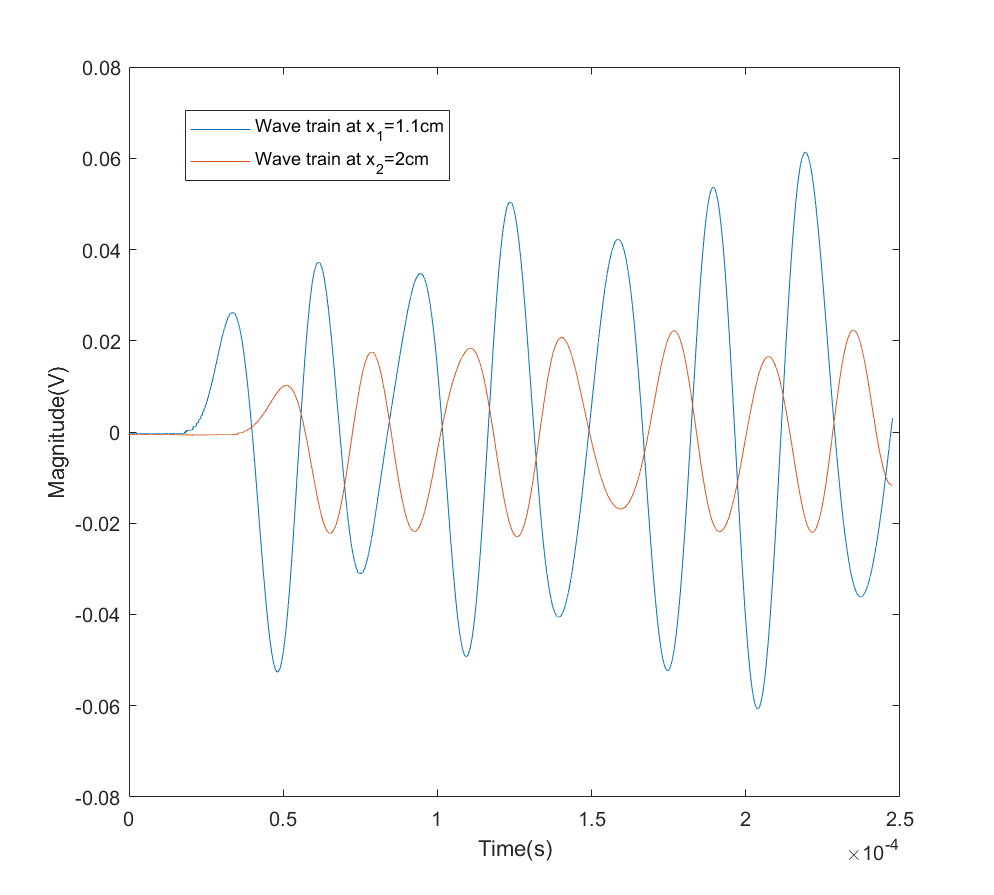
\includegraphics[height=6cm]{figures/2_wave_train.png}}
  \hspace{1cm}
  \bisubcaptionbox{$0-60\unit{kHz}$ 的相速度频域分布热图}{Phase velocity frequency distribution heat map at $0-60\unit{kHz}$}%
                [7cm]{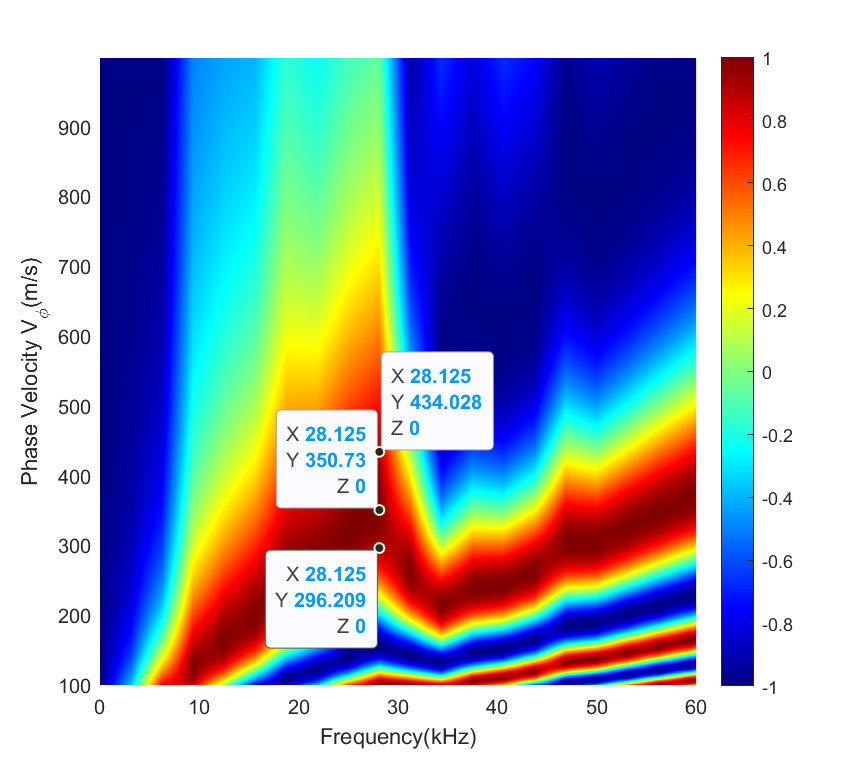
\includegraphics[height=6cm]{figures/2_cwt_v_phi.png}}
  \bicaption{根据异地响应信号计算频散能量图}{Dispersion energy map calculated from separated response signals}
  \label{fig:dispersion_energy}
\end{figure}

图 \ref{fig:dispersion_energy} 展示了在单轴应力容器中,根据不同采集距离下的两道压缩波信号绘制的频散能量图。可以看到两道信号在发射信号的中心频率 $f_{c} = 30\text{ kHz}$ 处的相速度约为 $V_{\varphi} = 350\pm 10\unit{m/s}$。

\section{声速与单轴应力的指数关系}

\subsection{等效介质理论(EMT)}

假定声波波长 $\lambda\gg$ 颗粒直径 $d$,颗粒体系由相同颗粒组成,满足紧束缚条件,颗粒介质应变可采用仿射近似,则纵波声速 $V_{L}$ 与横波声速 $V_{T}$ 分别为

\begin{align}
  V_{L} &= \sqrt{\frac{(K+\frac{4}{3}G)}{\rho^{*}}},\\
  V_{T} &= \sqrt{\frac{G}{\rho^{*}}},
\end{align}

其中 $K$ 与 $G$ 分别是颗粒介质的体弹性模量与剪切弹性模量,$\rho^{*}=\rho\phi$ 是颗粒固体的密度,$\rho$ 是颗粒材料的密度,$\phi$ 是颗粒的体积分数。在 EMT 中 模量如下给出:

\begin{align}
  K &= \frac{C_{n}}{12\uppi}\left(\phi Z\right)^{\frac{2}{3}}\left(\frac{6\uppi P}{C_{n}}\right)^{\frac{1}{3}},\\
  G &= \frac{C_{n} + \frac{3}{2}C_{t}}{20\uppi}\left(\phi Z\right)^{\frac{2}{3}}\left(\frac{6\uppi P}{C_{n}}\right)^{\frac{1}{3}},
\end{align}

其中 $Z$ 是颗粒的平均接触数,$C_{n}$、$C_{t}$ 分别是描述颗粒在法向和切向与力相关的系数。Hertz 接触和 Mindlin 接触分别使用了这两个系数,即两个颗粒通过接触完成的相互作用为

\begin{align}
  f_{n} &= \frac{2}{3}C_{n}R^{\frac{1}{2}}w^{\frac{3}{2}},\\
  f_{t} &= C_{t}(Rw)^{\frac{1}{2}}\Delta s,
\end{align}

其中 $w$ 是半径分别为 $R_{1}$、$R_{2}$ 的两个颗粒之间的重叠量,$R = \frac{2R_{1}R_{2}}{R_{1} + R_{2}}$ 为颗粒的等效半径。引入颗粒材料(下标 $g$)的剪切模量 $G_{g}$ 与泊松比 $\nu_{g}$,完成对力系数的表述:

\begin{align}
  C_{n} &= \frac{4G_{g}}{1-\nu_{g}},\\
  C_{t} &= \frac{8G_{g}}{2-\nu_{g}}.
\end{align}

\subsection{实验验证}\label{sec:stress_velocity_relation}

同样在单轴应力容器装置中,使用直径 $d=2\unit{\milli\meter}$ 的钢珠制备随机密堆积,并施加单轴应力 $P=$ \numlist{0.40;3.34;6.30;8.43;9.63;11.31;14.46}\unit{\kilo\pascal}。使用飞行时间法测定各应力下的声速 $V_{\text{T.O.F.}}(P)$,并观察声速与单轴应力的指数关系是否符合 EMT 的预期。

\begin{figure}[!hbtp]
  \centering
  \bisubcaptionbox{双线性轴下的应力 $P$ 与声速 $V_{\text{T.O.F.}}$ 的关系}%
                  {Stress $P$ versus sound velocity $V_{\text{T.O.F.}}$ in bilinear axis}%
                  [6.4cm]{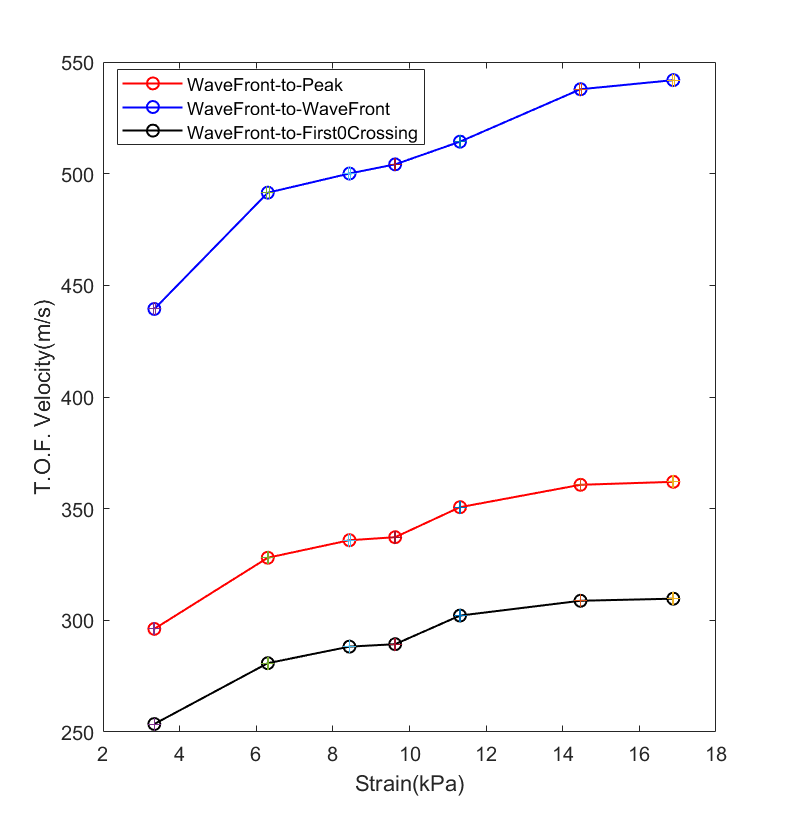
\includegraphics[height=7cm]{figures/2_strain_vs_velocity_20mm_1.png}}
  \hspace{1cm}
  \bisubcaptionbox{双对数处理后的应力 $P$ 与声速 $V_{\text{T.O.F.}}$ 的关系及其线性拟合}%
                  {Relationship between stress $P$ and sound velocity $V_{\text{T.O.F.}}$ after double logarithmic  and its linear fit}%
                  [6.4cm]{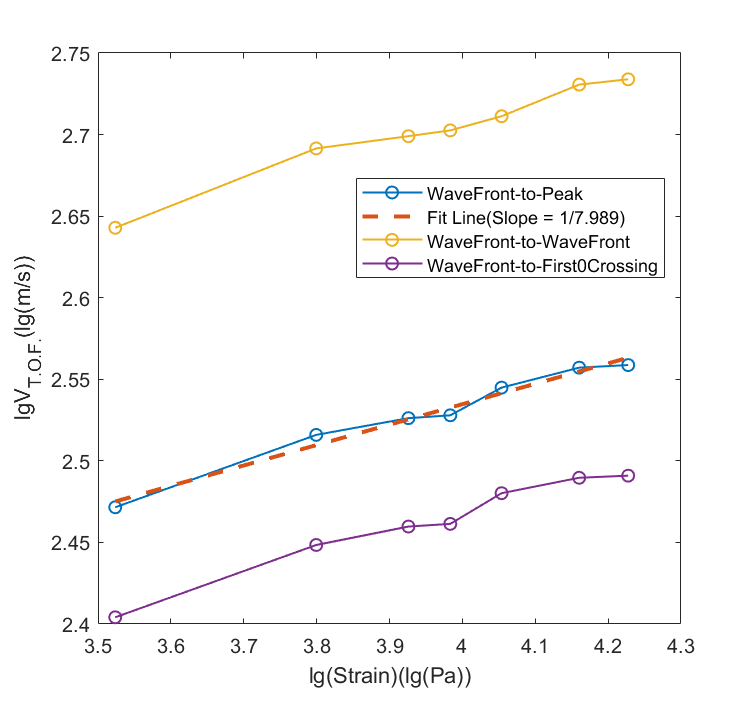
\includegraphics[height=7cm]{figures/2_strain_vs_velocity_20mm_2.png}}
  \bicaption{声速 $V_{\text{T.O.F.}}$ 与单轴应力 $P$ 的幂律关系。$P =$ \numlist{0.40;3.34;6.30;8.43;9.63;11.31;14.46}\unit{\kilo\pascal},颗粒介质为厚度 $L =19$\unit{\milli\meter} 的直径 $2$\unit{\milli\meter} 钢珠随机密堆积}
                  {Power-law relationship between the sound velocity $V_{\text{T.O.F.}}$ and the uniaxial stress $P$. $P =$ \numlist[
                    list-final-separator = { and }
                  ]{0.40;3.34;6.30;8.43;9.63;11.31;14.46}\unit{\kilo\pascal}, where the granular medium is a random close packing with steel beads of diameter $2\unit{\milli\meter}$ and thickness $L = 19$\unit{\milli\meter}}
  \label{fig:normalized_width_versus_L}
\end{figure}


%%% 可能是因为容器几何因素导致的 Yassen Effect,导致应力并不充分地施加到颗粒介质上。

\section{超声脉冲在颗粒介质中的展宽}

颗粒介质通过异质性的力链网络传递应力,因此声波在颗粒介质中传播时会因为其非线性出现剧烈的畸变现象,其中脉冲超声波的展宽是较为明显的现象之一。本节讨论了颗粒介质厚度 $L$ 以及单轴应力 $P$ 对于脉冲波展宽的影响。

\subsection{归一化宽度的定义}

在信号处理中,常见的对于峰宽度的定义通常是半高宽;事实上,我们在处理响应信号的到达时间时,使用的寻峰算法中的参数也的确包含了半高宽阈值用于排除噪音的干扰。但是这里我们引入的归一化宽度参数 $W$ 同时考虑了峰值与波前在时域中位置:

\begin{equation}
  W \equiv \frac{t_{1}-t_{0}}{t_{1}},
\end{equation}

其中 $t_{0}$ 与 $t_{1}$ 分别为波前与峰值的到达时间。我们在测定最佳信号参考点的时候应当意识到,脉冲的展宽实际上已经在一定程度上反映了“在颗粒介质中存在着较明显的色散关系”;而峰值到达时间定义的飞行时间速度,即在试探信号中心频率附近,在距离上更具有稳定性。因此,通过与中心频率(这里指所发射的试探信号的频率 $f_{c}$)关联的 $t_{1}$ 来对信号进行缩放操作是合理的。后文通过数据处理后得到的图~\ref{fig:reference_point} 以及对应讨论中进一步证明这一点。

\subsection{归一化宽度与颗粒介质厚度的关系}

\subsubsection{理论推导}

我们先从最简单的一维弹簧链开始推导。凝聚态物理中,我们已经知道一维晶格的色散关系为

\begin{equation}
  \omega=\sqrt{\frac{4C}{M}}\left|\sin\left(\frac{ka}{2}\right)\right|,
\end{equation}

其中 $C$ 为弹性系数,$M$ 为弹簧所连接质点的质量,$a$ 为质点间距/晶格常数。我们将其写为反函数形式:

\begin{equation}
  k(\omega) = \frac{2}{a}\arcsin{\left(\sqrt{\frac{M}{4C}}\omega\right)}.\label{eq:1D_dispersion_relation}
\end{equation}

在这里,我们对式~\eqref{eq:1D_dispersion_relation} 应用长波极限 $ka\ll 1$, 从而求得波速度:

\begin{equation}
  V = \lim_{ka\ll 1}\frac{\omega}{k} = \sqrt{\frac{C}{M}}a.
\end{equation}

使用 $V$ 替换式~\eqref{eq:1D_dispersion_relation} 中的 $C$,$M$ 项,且假定长波极限下的声速 $V$ 充分大,使得我们足以通过麦克劳林级数将其展开至前两项:

\begin{equation}
  k = \frac{2}{a}\left[\frac{a\omega}{2V} + \frac{1}{6}\left(\frac{a\omega}{2V}\right)^{3} + o\left(\frac{1}{V^3}\right)\right]\approx\frac{\omega}{V} + \frac{2\omega^{3}a^{2}}{3V^{3}},
\end{equation}

将其代入至波数项中,我们将看到

\begin{equation}
  \text{exp}\left[{\ii \left(\frac{\omega}{V} + \frac{2a^{2}\omega^{3}}{3V^{3}}\right)x}\right] = \text{exp}[{\ii\omega t_{1}}]\text{exp}\left[{\ii\left(\frac{\omega}{\omega_{1}}\right)^{3}}\right],\quad t_{1} = \frac{x}{V},\quad \omega_{1} = \sqrt[3]{\frac{3V^{3}}{2a^{2}x}}.\label{eq:rescale_method}
\end{equation}

而我们已经知道,在傅里叶变换中,存在关系

\begin{align}
  \mathcal{F}[f(t+t_{1})] = \mathcal{F}[f(t)]{\ee}^{\ii\omega t_{1}},\label{eq:translation_property}\\
  \mathcal{F}[f(\omega_{1}t)] = \frac{1}{|\omega_{1}|}\hat{f}\left(\frac{\omega}{\omega_{1}}\right),\label{eq:scale_property}\\
  \mathcal{F}[\text{Ai}(t)] = \text{exp}\left[\ii\cdot \frac{1}{3}\omega^3\right].
\end{align}

将波数项代入至 $a(x,-t)$ 中,并对其进行傅里叶变换:

\begin{equation}
  \mathcal{F}[a(x,-t)] = \int_{-\infty}^{+\infty}A_{0}{\ee}^{\ii\omega t_{1}}{\ee}^{\ii(\omega/\omega_{1})^{3}}e^{\ii\omega t}e^{-\ii\omega t}\mathrm{d}t = A_{0}{\ee}^{\ii\omega t_{1}}{\ee}^{\ii(\omega/\omega_{1})^{3}}.
\end{equation}

所以,根据傅里叶变换的平移性质~\eqref{eq:translation_property}与尺度性质~\eqref{eq:scale_property},我们得到源信号形式可近似为通过 $\omega_{1}$ 控制宽度的 Airy 函数:

\begin{equation}
  s(x,t) = \omega_{1}\text{Ai}\left[\omega_{1}(t_{1}-t)\right].
\end{equation}

因此,在一维弹簧链中,脉冲波传播到距离 $L$ 处的归一化宽度为

\begin{equation}
  W \approx \frac{\pi}{2\omega_{1}}\frac{1}{t_{1}}\propto L^{-2/3}.
\end{equation}

考虑一维球链时,使用 $a=2R$ 替换即可得到对应的公式\cite{PhysRevE.91.022205}。接下来我们进一步考虑颗粒介质中衰减项 $\alpha$ 的影响。引入弹性模量的涨落 $\nu_{K} = \Delta K^{-1}/\bar{K}^{-1}$ 与对应的关联长度 $L_{c}$,我们可以得到一维随机层理论对于衰减项的描述:

\begin{equation}
  \alpha(\omega) = k^{\prime\prime}(\omega) = [\sigma_{K}^{2}L_{c}^{n-1}]\left(\frac{\omega}{V}\right)^{n}.
\end{equation}

其中满足

\begin{align}
  V &= \bar{V} = \sqrt{\frac{\bar{K}}{\bar{\rho}}}\\
  \gamma &= \int_{0}^{+\infty}\langle\nu_{K}(0)\nu_{K}(x)\rangle\mathrm{d}x = \sigma_{K}^{2}L_{c}
\end{align}

通过引入虚波矢 $k^{\prime\prime}$ 写出频域内的信号分布,并仿照上面一维弹簧链中的式~\eqref{eq:rescale_method} 进行缩放操作:

\begin{equation}
  \widetilde{a}(\omega) = {\ee}^{ik^{\prime}x}e^{-k^{\prime\prime}x} = e^{i\omega t_{1}}e^{-\left(\frac{\omega}{\omega_{1}}\right)^{n}},\quad t_{1} = \frac{x}{V},\quad \omega_{1} = \sqrt[n]{\frac{V^{n}}{\sigma_{K}^{2}L_{c}^{n-1}x}}.
\end{equation}

因此得到归一化宽度:

\begin{equation}
W\sim \frac{1}{\omega_{1}t_{1}} = (\sigma_{K})^{\frac{2}{n}}\left(\frac{n-1}{n}\right)^{\frac{n-1}{n}}
\end{equation}

在一维随机分层介质中有 $n=2$, 因此在 $x = L$ 处归一化宽度为

\begin{equation}
  W\propto L^{-\frac{1}{2}}.
\end{equation}

\subsubsection{实验验证}

我们控制试探信号为 $5$ 循环 $30\unit{\kilo\Hz}$ 连续正弦波列作为试探信号,使用颗粒为直径 $2\unit{\milli\meter}$ 的钢珠生成随机密堆积,施加的单轴应力为 $9\unit{\kilo\Pa}$;分别测定了颗粒介质厚度为 $\numlist{6;11;16;20;24;30}\unit{\milli\metre}$ 时的响应信号,并且每一厚度都各自单独重新制备 7 次随机密堆积以尽可能消除实验误差,并且数据进行系综平均,标准差作为误差棒。图~\ref{fig:reference_point} 展示了其中一组响应信号通过相干波峰 $A_{1}$ 归一化,且时间轴以波峰到达时间 $t_{1}$ 进行缩放后的图像:

\begin{figure}[!htp]
  \centering
  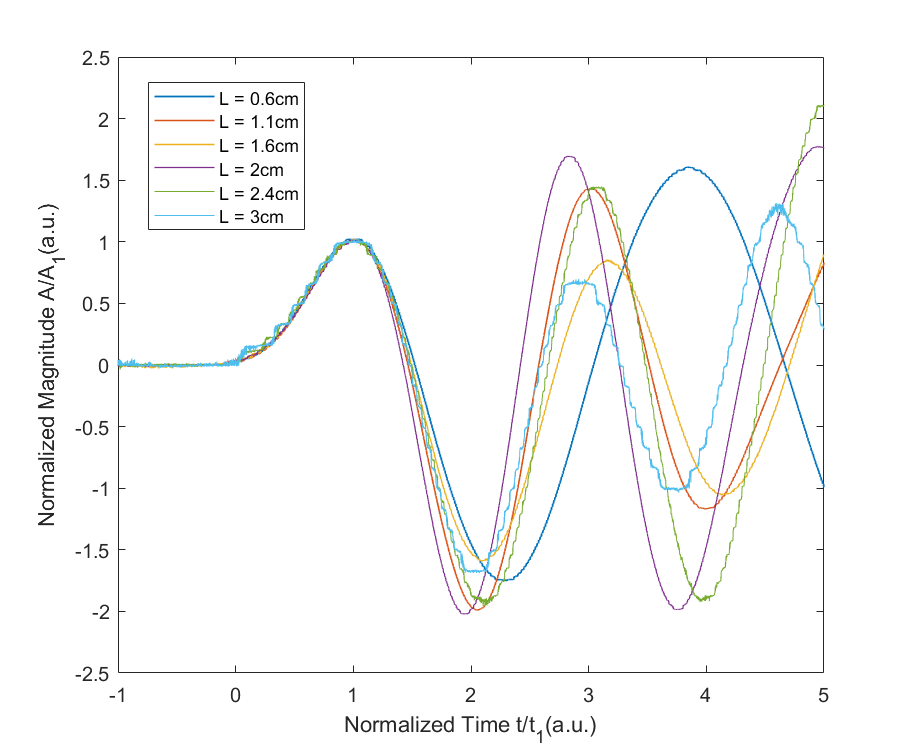
\includegraphics[height=6cm]{2_Rescaled_Magnitude_differing_in_Distance.png}
  \bicaption{通过相干波峰 $A_{1}$ 归一化,且时间轴以波峰到达时间 $t_{1}$ 进行缩放后的不同颗粒样品厚度下测得的响应信号}{Response signal captured at different granular sample thicknesses, normalized with coherent wave peak $A_{1}$ and time axis rescaled with peak arrival time $t_{1}$}
  \label{fig:reference_point}
\end{figure}

可以发现,虽然采集信号时的颗粒介质厚度各异,但是通过幅值归一化与时间轴的缩放,仍能够观察到“响应信号可以提取出相干首波”的本质特征。当 $t/t_{1} > 1$,响应信号的宽度开始出现显著变化;而在前面的信号参考点选取的实验中,我们已经知道,$t_{1}$ 是一个性质较为良好的参考点,因此我们可以通过借助 $t_{1}$ 定义的归一化宽度 $W$ 来探究其与颗粒介质厚度,即信号传播距离 $L$ 之间的关系。

图~\ref{fig:normalized_width_versus_L} 展示了上述实验中测得的归一化宽度 $W$ 与颗粒介质厚度 $L$ 之间的关系,其中为了观察幂律关系使用了双对数处理并对其数据点进行了线性拟合。不难看出,我们得出的结果约为 $W\propto L^{-0.448}$,与理论推导的 $W\propto L^{-1/2}$ 已经相当接近。

需要说明的是,这种偏差存在两种来源:

\begin{enumerate}
  \item 波前到达时间的选取并不是绝对的。既然我们是通过 $S(t_{0}) = A_{1}\cdot k$($k\in(0,0.1]$)确定的 $t_{0}$,那么 $k$ 的具体数值会影响到 $t_{0}$ 的选取,从而影响到归一化宽度 $W$ 的测定;而在传播距离较大时,响应信号的信噪比会因为信号衰减而急剧降低,此时对全体传播距离上的响应信号划定一条通用可行的 $k$ 实际上是存在困难的,因此其具体数值需要通过经验来调整;
  \item 理论推导中的 $n=2$ 是一维随机分层介质的情况。虽然我们已经将色散关系和衰减同时纳入考虑,并且实验模式中超声波的传播偏向于柱坐标中单个 $z$ 轴方向上,但是着一切仍不能改变“实际的颗粒介质仍然是三维体系”的事实,因此出现 $-0.448\sim-1/2$ 的偏差是在理解范围内的。
\end{enumerate}

\begin{figure}[!hbtp]
  \centering
  \bisubcaptionbox{相干首波峰宽度 $t_{1} - t_{0}$}%
                  {Coherent wave peak width $t_{1} - t_{0}$}%
                  [6.4cm]{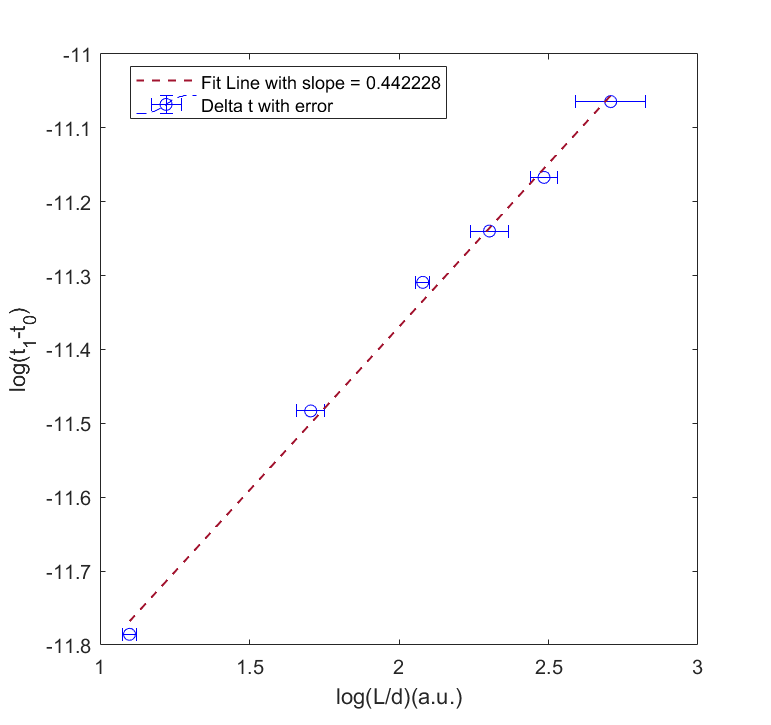
\includegraphics[height=7cm]{figures/2_t1-t0_L.png}}
  \hspace{1cm}
  \bisubcaptionbox{相干首波归一化宽度 $W$}%
                  {Coherent first wave normalized width $W$}%
                  [6.4cm]{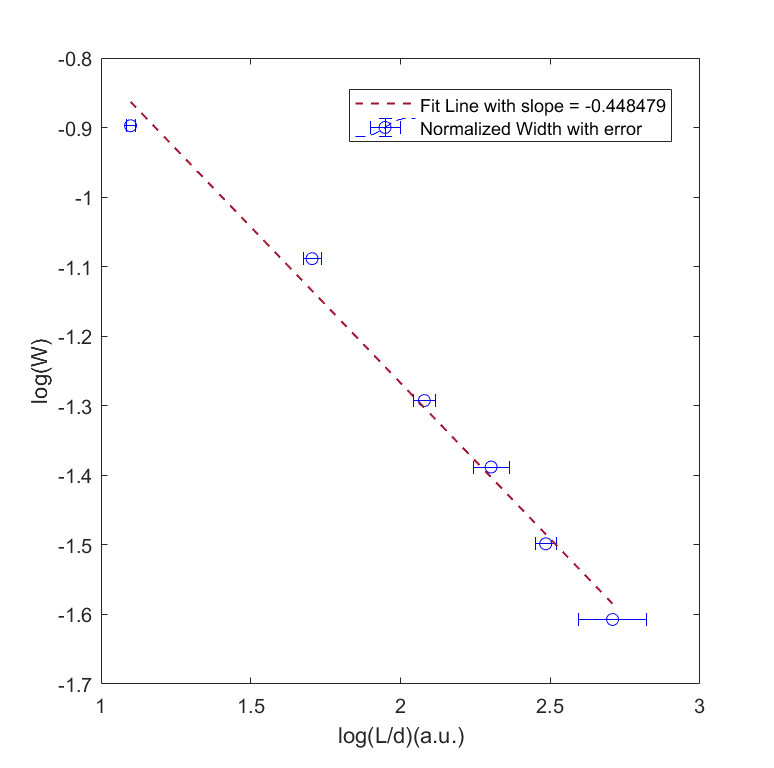
\includegraphics[height=7cm]{figures/2_W_L.png}}
  \bicaption{颗粒介质厚度为 \numlist{6;11;16;20;24;30} \unit{\milli\metre} 时的响应信号首峰宽度 $t_{1} - t_{0}$ 与归一化宽度 $W$}
                  {First peak width $t_{1} - t_{0}$ and normalized width $W$ of response signal at granular medium thickness of \numlist[
                    list-final-separator = { and }
                  ]{6;11;16;20;24;30} \unit{\milli\metre}}
  \label{fig:normalized_width_versus_L}
\end{figure}

\subsection{归一化宽度与单轴应力的关系}

类似于上述实验中考虑的颗粒介质厚度,即脉冲传播距离 $L$ 对脉冲归一化宽度 $W$ 的影响,我们也对在不同单轴应力 $P$ 下的归一化宽度 $W(P)$ 进行了计算与绘图,数据来自于小节~\ref{sec:stress_velocity_relation} 中单轴应力与声速关系的实验。但遗憾的是,如图~\ref{fig:normalized_width_versus_P} 所示,我们没有观察到两者之间存在着任何明显的规律。

\begin{figure}[!hbtp]
  \centering
  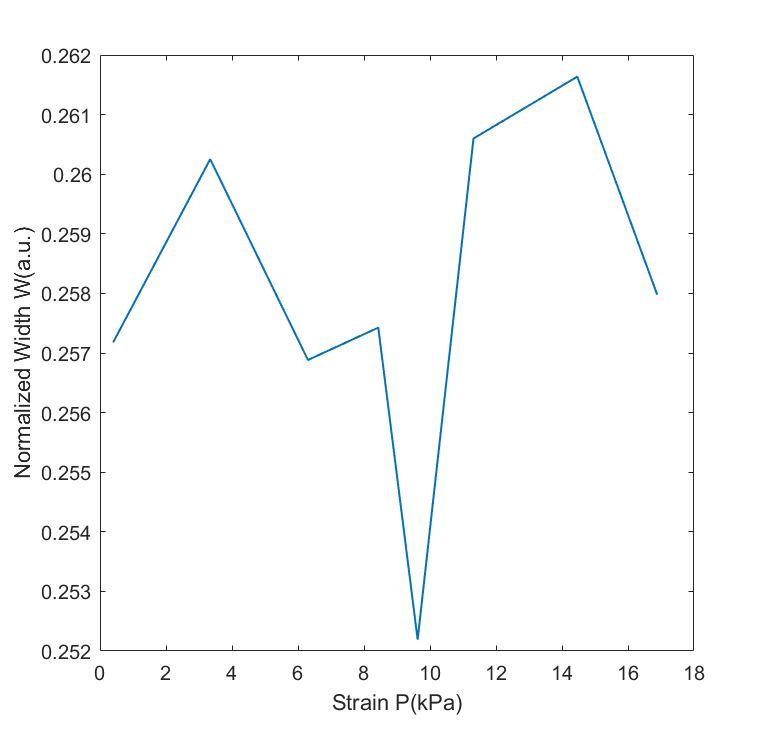
\includegraphics[height=7cm]{figures/2_W_norm&Strain.png}
  \bicaption{单轴应力 $P$ 与归一化宽度 $W$ 的关系}{Relationship between uniaxial stress $P$ and normalized width $W$}
  \label{fig:normalized_width_versus_P}
\end{figure}

目前对于该现象的解释是,颗粒介质中本身存在着如 Jassen Effect 等现象,即在诸如圆筒形容器中颗粒介质所受重力并非完全沿轴向传递,而是会有一部分力被颗粒介质中的结构分配到径向。这与通常的液压规律完全不同,因此早期人类的粮仓会因为设计不合理而被过量的径向应力破坏、坍塌\cite{sperlExperimentsCornPressure2006}。在我们的实验中,由于容器的几何因素,可能类似的效应使得颗粒介质对于脉冲信号的响应规律性受到影响,导致所观察到的 $W(P)$ 与 $P$ 之间的关系并不明显。